\label{sec:backgrounds}
%% An accurate description of the background process is an essential aspect of any analysis since it affects the extraction of signal yields.
The main background sources differ between the three channels, but can be divided into two categories.

In the first one there are processes which have the same final state as the signal and survive all signal region cuts (\textit{irreducible background}).
These are processes that generate the same stable particles as the signal,
although the kinematic distributions may be different.
Usually processes in this class are estimated with simulation,
but in some cases it is possible to constrain their normalization in a control region.

In the second one fall processes that have a different final state than the signal, but enter in the signal region nonetheless (\textit{reducible background}).
Although the final states are different,
either due to additional particles produced in the same hard scattering
or coming from other collisions in the same bunch crossing (\pileup),
that are reconstructed in the detector and not rejected by the identification algorithms,
they generate events which pass the selection.
This particles can either be \nonprompt leptons or photons, or misidentified light-flavour jets.

\Nonprompt leptons come mainly from decays of heavy flavour mesons and electrons from asymmetric photons conversions,
while \nonprompt photons originate primarily from decays of light neutral mesons like \PGpz or \PGh.
Both leptons and photons in this category tend to be non-isolated from the nearby jet activity.

The other class is comprised of misidentified jets, mostly from light-flavour quarks, which can erroneously be reconstructed as either leptons,
if a track is associated with the main energy deposits, or as photons otherwise.
These misidentified photons tend to have a different energy distribution in the ECAL with respect to real photons,
which makes shower shape variables effective in separating this background from real photons.

In the following the terms \textit{fake leptons} and \textit{fake photons} are used to refer to both \nonprompt and misidentified objects.
These processes have cross sections orders of magnitude larger than the signal.
Often these backgrounds prove difficult to model in simulation,
and it becomes advisable to use a data-driven method for their estimation.

\subsection{Four lepton channel}
For the 4\Pl channel the predominant background component is the production of two on-shell \PZ bosons
which decay to either electrons or muons.
It is possible that a photon that is radiated as FSR from one of the leptons
is also present in the event, thus producing the same signature as the signal.
Alternatively the photon may be \nonprompt or a misreconstructed jet.

Two \PZ bosons can be produced through quark-antiquark annihilation, as shown in Figure~\ref{fig:qqtoZZto4L}
or from gluon fusion with a quark loop, illustrated in Figure~\ref{fig:ggtoZZto4L}.
The latter is a Next-to-Leading Order (NLO) process, and its contribution is around 10\usep\% of the former in terms of event yield.

Additional backgrounds such as $\PQt\PAQt\PZ$ and VVV (V = \PZ, \PW) result in very small contributions.

\begin{figure}
\hfill
\subfigure [$\PQq\PAQq \to \PZ\PZ \to 4\Pl$]     {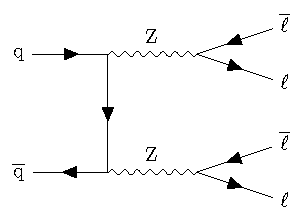
\includegraphics[width=.4\textwidth]{Figures/Feynman/qq_ZZ_4L.pdf} \label{fig:qqtoZZto4L}} \hfill
\subfigure [$\Pg\Pg \to \PZ\PZ \to 4\Pl$ (loop)] {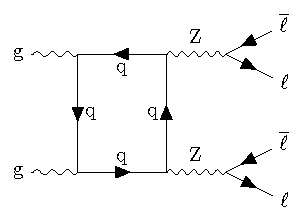
\includegraphics[width=.4\textwidth]{Figures/Feynman/gg_ZZ_4L.pdf} \label{fig:ggtoZZto4L}} \hfill\mbox{}
\caption{Feynman diagrams for the production of two Z bosons
with subsequent decay to four charged leptons
either from quark-antiquark annihilation
or from a gluon-initiated loop.}
\end{figure}

\subsection{Three lepton channel}
In the three lepton channel the main background contributions are $\PW\PZ$, Drell-Yan + jets and $\PZ\PGg$ + jets.
As for the $\PZ\PZ$ in the four lepton channel, in $\PW\PZ$ events an additional photon may be emitted as FSR from one of the leptons
or be a misidentified or \nonprompt particle.
The cross sections of Drell-Yan processes and $\PZ\PGg$ production are much larger than that of the signal and,
although the probabilities of particle misreconstruction or misidentification are comparatively small,
they result in a significant yield in the signal region.

Another not negligible contribution is the $\PZ\PZ \to 4\Pl$ where one of the leptons is lost or misreconstructed as a photon.
There is also a small fraction of events from $\PZ\PZ\PGg$ in which one of the leptons is outside the detector acceptance.
Additional backgrounds from rare processes such as $\PQt\PAQt\PZ$ and VVV (V = \PZ, \PW) result in very small contributions and are estimated with simulation.

\subsection{Two lepton channel}
In the two lepton channel the major background are Drell-Yan processes and $\PZ\PGg$ production.
Unlike the three lepton channel, the absence of the requirements on the presence of the third lepton and of the missing energy
enhances the contributions from these sources.
The main distinguishing feature is the kinematics and characteristics of the hadronic part of the events,
which plays a major role in this channel.
